\documentclass[border=8pt]{standalone}
\usepackage[utf8]{inputenc}
\usepackage{nacal}
\usepackage{tikz}
\usepackage{tikz-3dplot}
\usetikzlibrary{calc,angles,positioning,intersections,quotes,decorations.markings,arrows.meta,decorations.pathreplacing}
\usepackage{tkz-euclide}
\def\Datos{green!40!gray}
\def\Ajuste{blue!50!red}
\def\Residuo{black!25!gray}
\def\Regresor{blue!75!white}
\def\Base{orange!80!black}
\def\Sistem{blue!50!black}
\tikzset{vector/.style={-{Stealth[length=3mm, width=2mm]},very thick},
         basevec/.style={-{Stealth[length=2.2mm, width=1.6mm]},thick,\Base},
         guide/.style={dashed,thin,gray}}

\begin{document}
  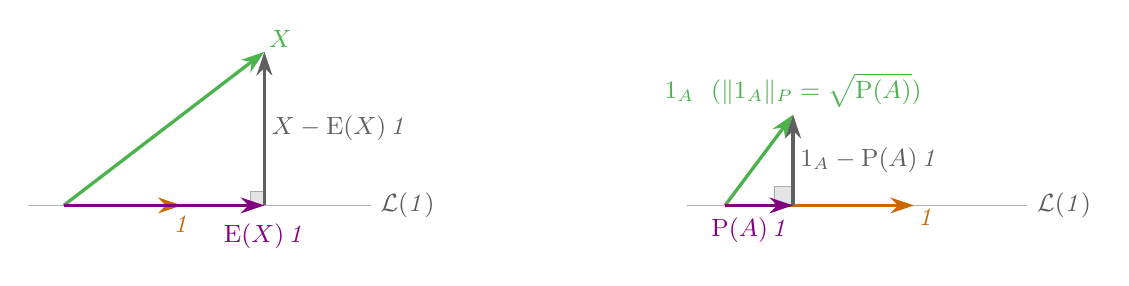
\begin{tikzpicture}[scale=1.5]
    % panel izquierdo: X
    \begin{scope}
      \coordinate (O) at (0,0); \coordinate (U) at (1,0); \coordinate (X) at (1.7,1.3); \coordinate (PX) at (1.7,0);
      \draw[gray!60,thin] (-0.3,0) -- (2.6,0) node[anchor=west,font=\small,gray!70!black] {$\mathcal L(\mathit1)$};
      \tkzMarkRightAngle[size=.12,gray,very thin,fill=lightgray!70,opacity=0.6](O,PX,X)
      \draw[vector,\Base] (O) -- (U) node[anchor=north,font=\small] {$\mathit1$};
      \draw[vector,\Datos] (O) -- (X) node[anchor=south west,font=\small,inner sep=1pt] {$X$};
      \draw[vector,\Ajuste] (O) -- (PX) node[pos=1,anchor=north,font=\small,yshift=-1mm] {$\mathrm E(X)\,\mathit1$};
      \draw[vector,\Residuo] (PX) -- (X) node[pos=0.5,anchor=west,font=\small,inner sep=2pt] {$X-\mathrm E(X)\,\mathit1$};
    \end{scope}
    % panel derecho: indicadora
    \begin{scope}[xshift=5.6cm,scale=1.6]
      \coordinate (O) at (0,0); \coordinate (U) at (1,0); \coordinate (A) at (0.36,0.48); \coordinate (PA) at (0.36,0);
      \draw[gray!60,thin] (-0.2,0) -- (1.6,0) node[anchor=west,font=\small,gray!70!black] {$\mathcal L(\mathit1)$};
      \tkzMarkRightAngle[size=.10,gray,very thin,fill=lightgray!70,opacity=0.6](O,PA,A)
      \draw[vector,\Base] (O) -- (U) node[anchor=north west,font=\small,inner sep=1pt] {$\mathit1$};
      \draw[vector,\Datos] (O) -- (A) node[anchor=south,font=\small,inner sep=2pt] {$\mathbb 1_A$ \ ($\Vert\mathbb 1_A\Vert_P=\sqrt{\mathrm P(A)}$)};
      \draw[vector,\Ajuste] (O) -- (PA) node[pos=1,anchor=north east,font=\small,yshift=-1mm,inner sep=1pt] {$\mathrm P(A)\,\mathit1$};
      \draw[vector,\Residuo] (PA) -- (A) node[pos=0.5,anchor=west,font=\small,inner sep=2pt] {$\mathbb 1_A-\mathrm P(A)\,\mathit1$};
    \end{scope}
  \end{tikzpicture}
\end{document}
